% ============================================
% EXPECTED RESULTS
% ============================================

\begin{frame}{Expected Results - [1] (Output Interface)}
    \begin{center}
        % Standard size for the main result image
        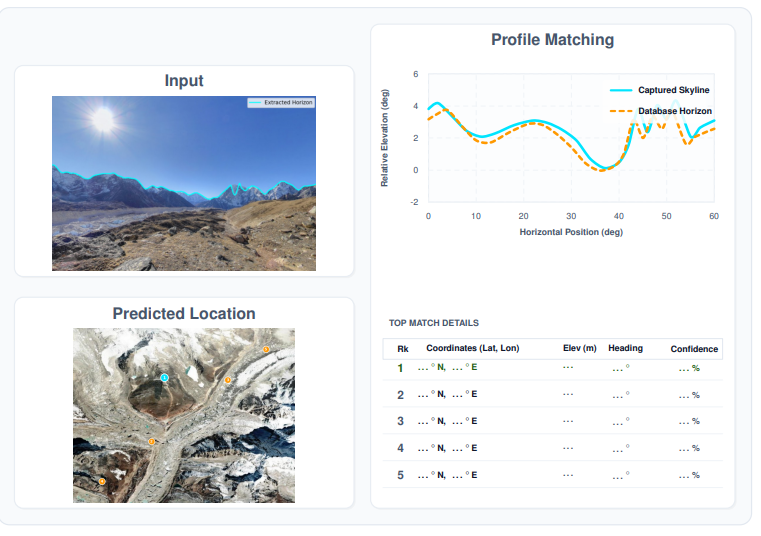
\includegraphics[width=0.85\textwidth, height=0.7\textheight, keepaspectratio]{src/images/page4.png} 
        \vfill
        \small \textbf{Figure:} Proposed interface showing predicted location on map and profile alignment.
    \end{center}
\end{frame}

\begin{frame}{Expected Results - [2] (Performance Metrics)}
    \begin{columns}[t, onlytextwidth]
        \begin{column}{0.55\textwidth}
            \textbf{Metrics for Evaluation:}
            \begin{itemize}
                \item \textbf{Top-$k$ Accuracy:} How often the ground-truth location appears in the top $1, 5, \text{ or } 10$ candidates.
                \item \textbf{Heading Error:} Angular difference between predicted and actual camera direction (limit: $\pm 0.25^\circ$).
                \item \textbf{Latency:} Time taken for FFT search and DTW refinement (Target: $< 2$ seconds).
            \end{itemize}
        \end{column}
        \begin{column}{0.42\textwidth}
            \begin{center}
                % If you have a PNG for this graph later, replace this \fbox with \includegraphics
                \fbox{\parbox{0.9\textwidth}{\centering
                    \vspace{1.5cm}
                    \small \textbf{[Expected Accuracy Graph]}\\
                    \tiny (Top-$k$ vs Success Rate)
                    \vspace{1.5cm}
                }}
            \end{center}
        \end{column}
    \end{columns}
\end{frame}

\begin{frame}{Expected Results - [3] (Robustness Analysis)}
    \begin{itemize}
        \item \textbf{Weather Resistance:} Performance evaluation across different visibility tiers (Clear, Moderate Haze, Dense Fog).
        \item \textbf{Focal Length Tolerance:} DTW's ability to handle stretching/compression from different smartphone lenses.
        \item \textbf{Memory Footprint:} Maintaining the $\sim 79$ MB database entirely in RAM for fast access.
    \end{itemize}
\end{frame}